\documentclass[UKenglish]{latex/atlasdoc}
\usepackage{latex/atlaspackage}
\usepackage{latex/atlasphysics}
\usepackage{latex/atlascontribute}

\usepackage{xspace}
\usepackage{multirow}
%\usepackage{verbatim}

\usepackage{makeidx}
\makeindex

\graphicspath{{logos/}{figures/}}


% Title, abstract and document 
%-------------------------------------------------------------------------------
% This file contains the title, author and abstract.
% It also contains all relevant document numbers used by the different cover pages.
%-------------------------------------------------------------------------------

% Title
\AtlasTitle{Associative Memory Boards Software Manual}

% Author - this does not work with revtex (add it after \begin{document})
\author[a]{Alberto Annovi}
\author[a]{Nicolò Biesuz}
\author[a]{Saverio Citraro}
\author[a]{Guido Volpi}

\affil[a]{Univ. and INFN Pisa}

% Authors and list of contributors to the analysis
% \AtlasAuthorContributor also adds the name to the author list
% Include package latex/atlascontribute to use this
% Use authblk package if there are multiple authors, which is included by latex/atlascontribute
% \usepackage{authblk}
% Use the following 3 lines to have all institutes on one line
% \makeatletter
% \renewcommand\AB@affilsepx{, \protect\Affilfont}
% \makeatother
% \renewcommand\Authands{, } % avoid ``. and'' for last author
% \renewcommand\Affilfont{\itshape\small} % affiliation formatting
% \AtlasAuthorContributor{First AtlasAuthorContributor}{a}{Author's contribution.}
% \AtlasAuthorContributor{Second AtlasAuthorContributor}{b}{Author's contribution.}
% \AtlasAuthorContributor{Third AtlasAuthorContributor}{a}{Author's contribution.}
% \AtlasContributor{Fourth AtlasContributor}{Contribution to the analysis.}
% \author[a]{First Author}
% \author[a]{Second Author}
% \author[b]{Third Author}
% \affil[a]{One Institution}
% \affil[b]{Another Institution}

% If a special author list should be indicated via a link use the following code:
% Include the two lines below if you do not use atlasstyle:
% \usepackage[marginal,hang]{footmisc}
% \setlength{\footnotemargin}{0.5em}
% Use the following lines in all cases:
% \usepackage{authblk}
% \author{The ATLAS Collaboration%
% \thanks{The full author list can be found at:\newline
%   \url{https://atlas.web.cern.ch/Atlas/PUBNOTES/ATL-PHYS-PUB-2016-007/authorlist.pdf}}
% }

% Date: if not given, uses current date
%\date{\today}

% Draft version:
% Should be 1.0 for the first circulation, and 2.0 for the second circulation.
% If given, adds draft version on front page, a 'DRAFT' box on top of each other page, 
% and line numbers.
% Comment or remove in final version.
\AtlasVersion{0.1}

% ATLAS reference code, to help ATLAS members to locate the paper
%\AtlasRefCode{GROUP-2016-XX}

% ATLAS note number. Can be an COM, INT, PUB or CONF note
% \AtlasNote{ATLAS-CONF-2016-XXX}
% \AtlasNote{ATL-PHYS-PUB-2016-XXX}
% \AtlasNote{ATL-COM-PHYS-2016-XXX}

% CERN preprint number
% \PreprintIdNumber{CERN-PH-2016-XX}

% ATLAS date - arXiv submission; to be filled in by the Physics Office
% \AtlasDate{\today}

% arXiv identifier
% \arXivId{14XX.YYYY}

% HepData record
% \HepDataRecord{ZZZZZZZZ}

% Submission journal and final reference
% \AtlasJournal{Phys.\ Lett.\ B.}
% \AtlasJournalRef{\PLB 789 (2014) 123}
% \AtlasDOI{}

% Abstract - % directly after { is important for correct indentation
\AtlasAbstract{%
	This document describes  the online software package used to
	control the associative memory board (AMB). 
	The software packages provides the ATLAS run control module,
	a library with low-level APIs, a collection of compiled tools  nd scripts
	used to control and monitor the board from a command line shell.
	
	Instructions on how to use the tools to monitor the road, perform
	base tests and solve eventual issues will be provided.
}

%-------------------------------------------------------------------------------
% The following information is needed for the cover page. The commands are only defined
% if you use the coverpage option in atlasdoc or use the atlascover package
%-------------------------------------------------------------------------------

% List of supporting notes  (leave as null \AtlasCoverSupportingNote{} if you want to skip this option)
% \AtlasCoverSupportingNote{Short title note 1}{https://cds.cern.ch/record/XXXXXXX}
% \AtlasCoverSupportingNote{Short title note 2}{https://cds.cern.ch/record/YYYYYYY}
%
% OR (the 2nd option is deprecated, especially for CONF and PUB notes)
%
% Supporting material TWiki page  (leave as null \AtlasCoverTwikiURL{} if you want to skip this option)
% \AtlasCoverTwikiURL{https://twiki.cern.ch/twiki/bin/view/Atlas/WebHome}

% Comment deadline
% \AtlasCoverCommentsDeadline{DD Month 2016}

% Analysis team members - contact editors should no longer be specified
% as there is a generic email list name for the editors
% \AtlasCoverAnalysisTeam{Peter Analyser, Susan Editor1, Jenny Editor2, Alphonse Physicien}

% Editorial Board Members - indicate the Chair by a (chair) after his/her name
% Give either all members at once (then they appear on one line), or separately
% \AtlasCoverEdBoardMember{EdBoard~Chair~(chair), EB~Member~1, EB~Member~2, EB~Member~3}
% \AtlasCoverEdBoardMember{EdBoard~Chair~(chair)}
% \AtlasCoverEdBoardMember{EB~Member~1}
% \AtlasCoverEdBoardMember{EB~Member~2}
% \AtlasCoverEdBoardMember{EB~Member~3}

% A PUB note has readers and not an EdBoard -- give their names here (one line or several entries)
% \AtlasCoverReaderMember{Reader~1, Reader~2}
% \AtlasCoverReaderMember{Reader~1}
% \AtlasCoverEdBoardMember{Reader~2}

% Editors egroup
% \AtlasCoverEgroupEditors{atlas-GROUP-2016-XX-editors@cern.ch}

% EdBoard egroup
% \AtlasCoverEgroupEdBoard{atlas-GROUP-2016-XX-editorial-board@cern.ch}


\newcommand{\AMBoard}{\texttt{AMBoard}\xspace}
\newcommand{\RCModule}{\texttt{ReadoutModule\_Ambslp}\xspace}

\begin{document}
	
\maketitle

\tableofcontents

\section{Introduction}
This document describes  the structure, working principle and use cases for
the online software package used to
control the associative memory board, then referred as AMB or AMBSLP.
The software is contained in the package
\hyperlink{https://svnweb.cern.ch/trac/atlastdaq/browser/FTK/ambslp?order=name}
	{FTK/ambslp}
and managed by the AMB team. Instruction on how to compile the
package within the ATLAS TDAQ software framework are provided elsewhere,
with all required details. Indeed, the following documentation assumes knowledge
on how to compile it and provide information for both users and developers,
in order to provide documentation on how to control the board and
add or maintain the main functionalities.

More specifically,
the software  package provides:
\begin{itemize}
  \item a library containing low level functions
  used to control the board;

	\item a module loaded by the ATLAS run control (RC) to control the board,
	associated with the board description within this framework, base monitoring
    tools and more;
    
	\item a set of standalone tools, as compiled programs and scripts,
	used to control and monitor the board from a command line shell.
\end{itemize} 

The document goals are to both support the experts to verify
the behavior of a board, fixing eventual issues, as well as the developer to
change to evolve the code. The document will also try to document
the RC related parts and standalone software.

An initial section will be devoted to document some basic features of the boards,
related to its working principle, related to firmware and electronic characteristics.
The following section will provide more detailed information on the software components
designed to allow a correct working of the board and allowing to control
in different scenarios.

\section{Associative board working principle and features}
\begin{figure}
\centering
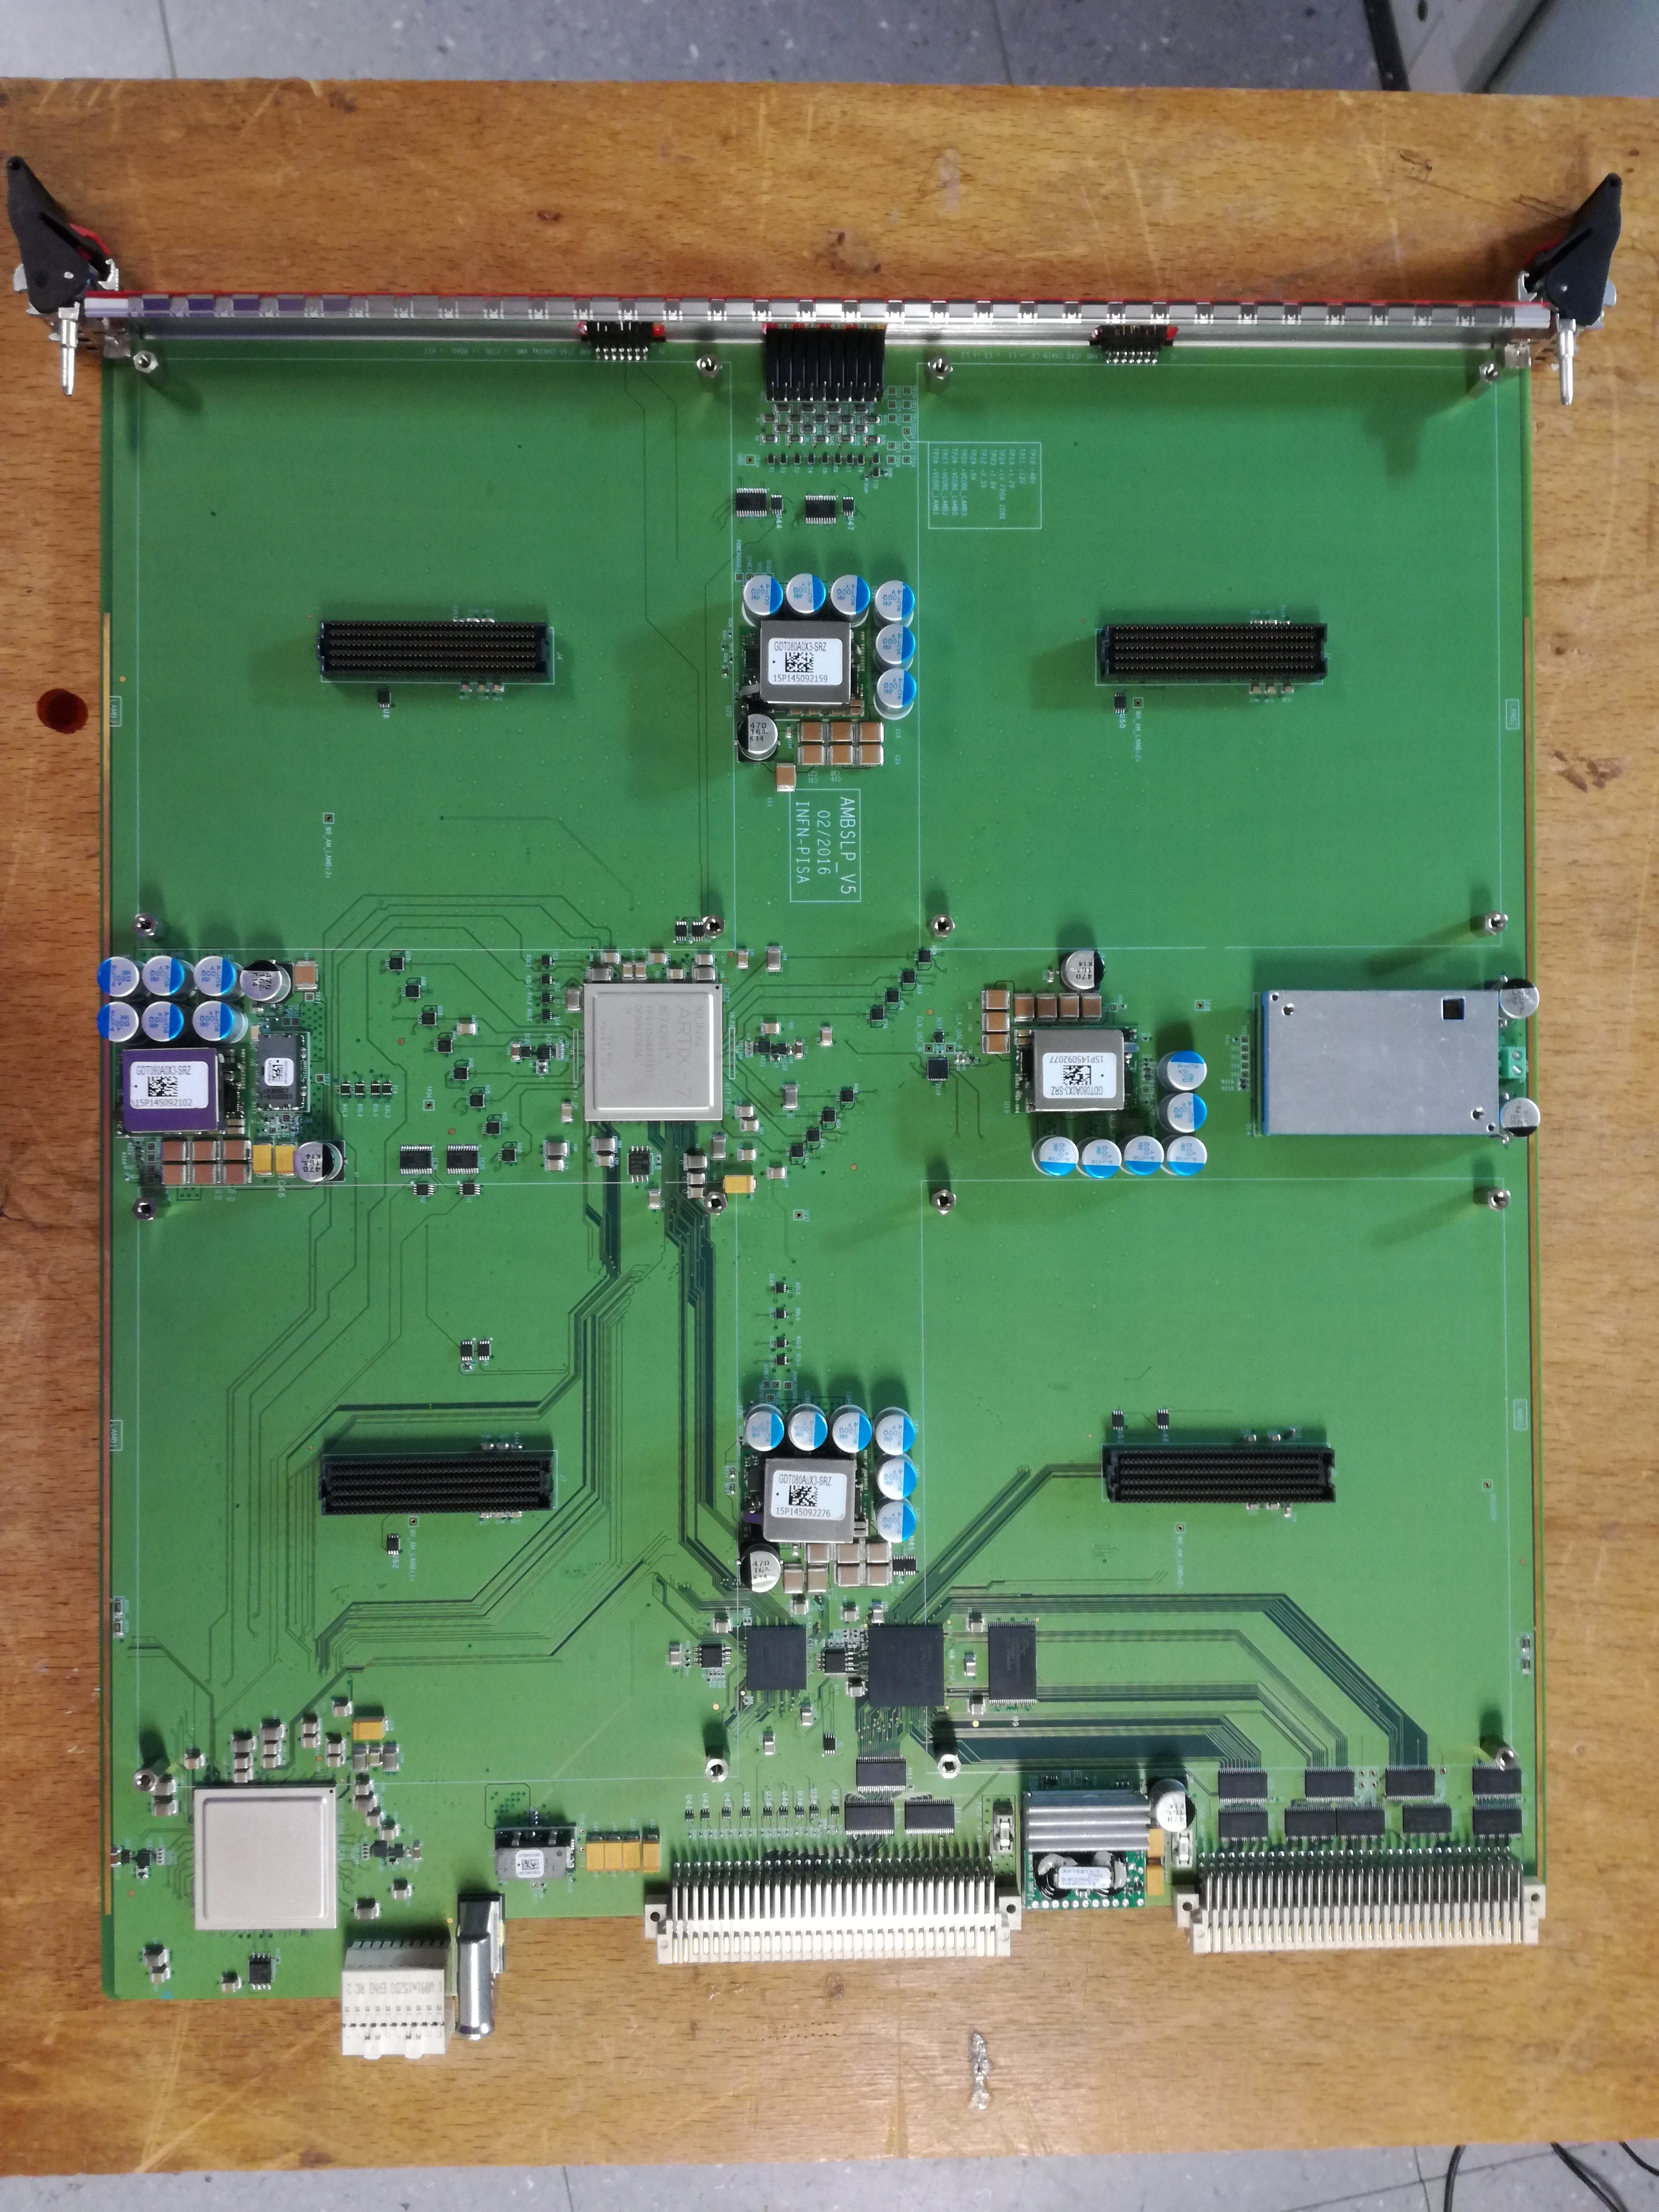
\includegraphics[width=.6\linewidth,angle=90]{Images/AMBoard.jpg}
\caption{The picture shows an AMBoard, top side. The 4 FPGAs are
clearly visible. The four FMC connectors show where the LAMBs wil be
installed}
\label{fig:amboard_top}
\end{figure}

\begin{figure}
\centering

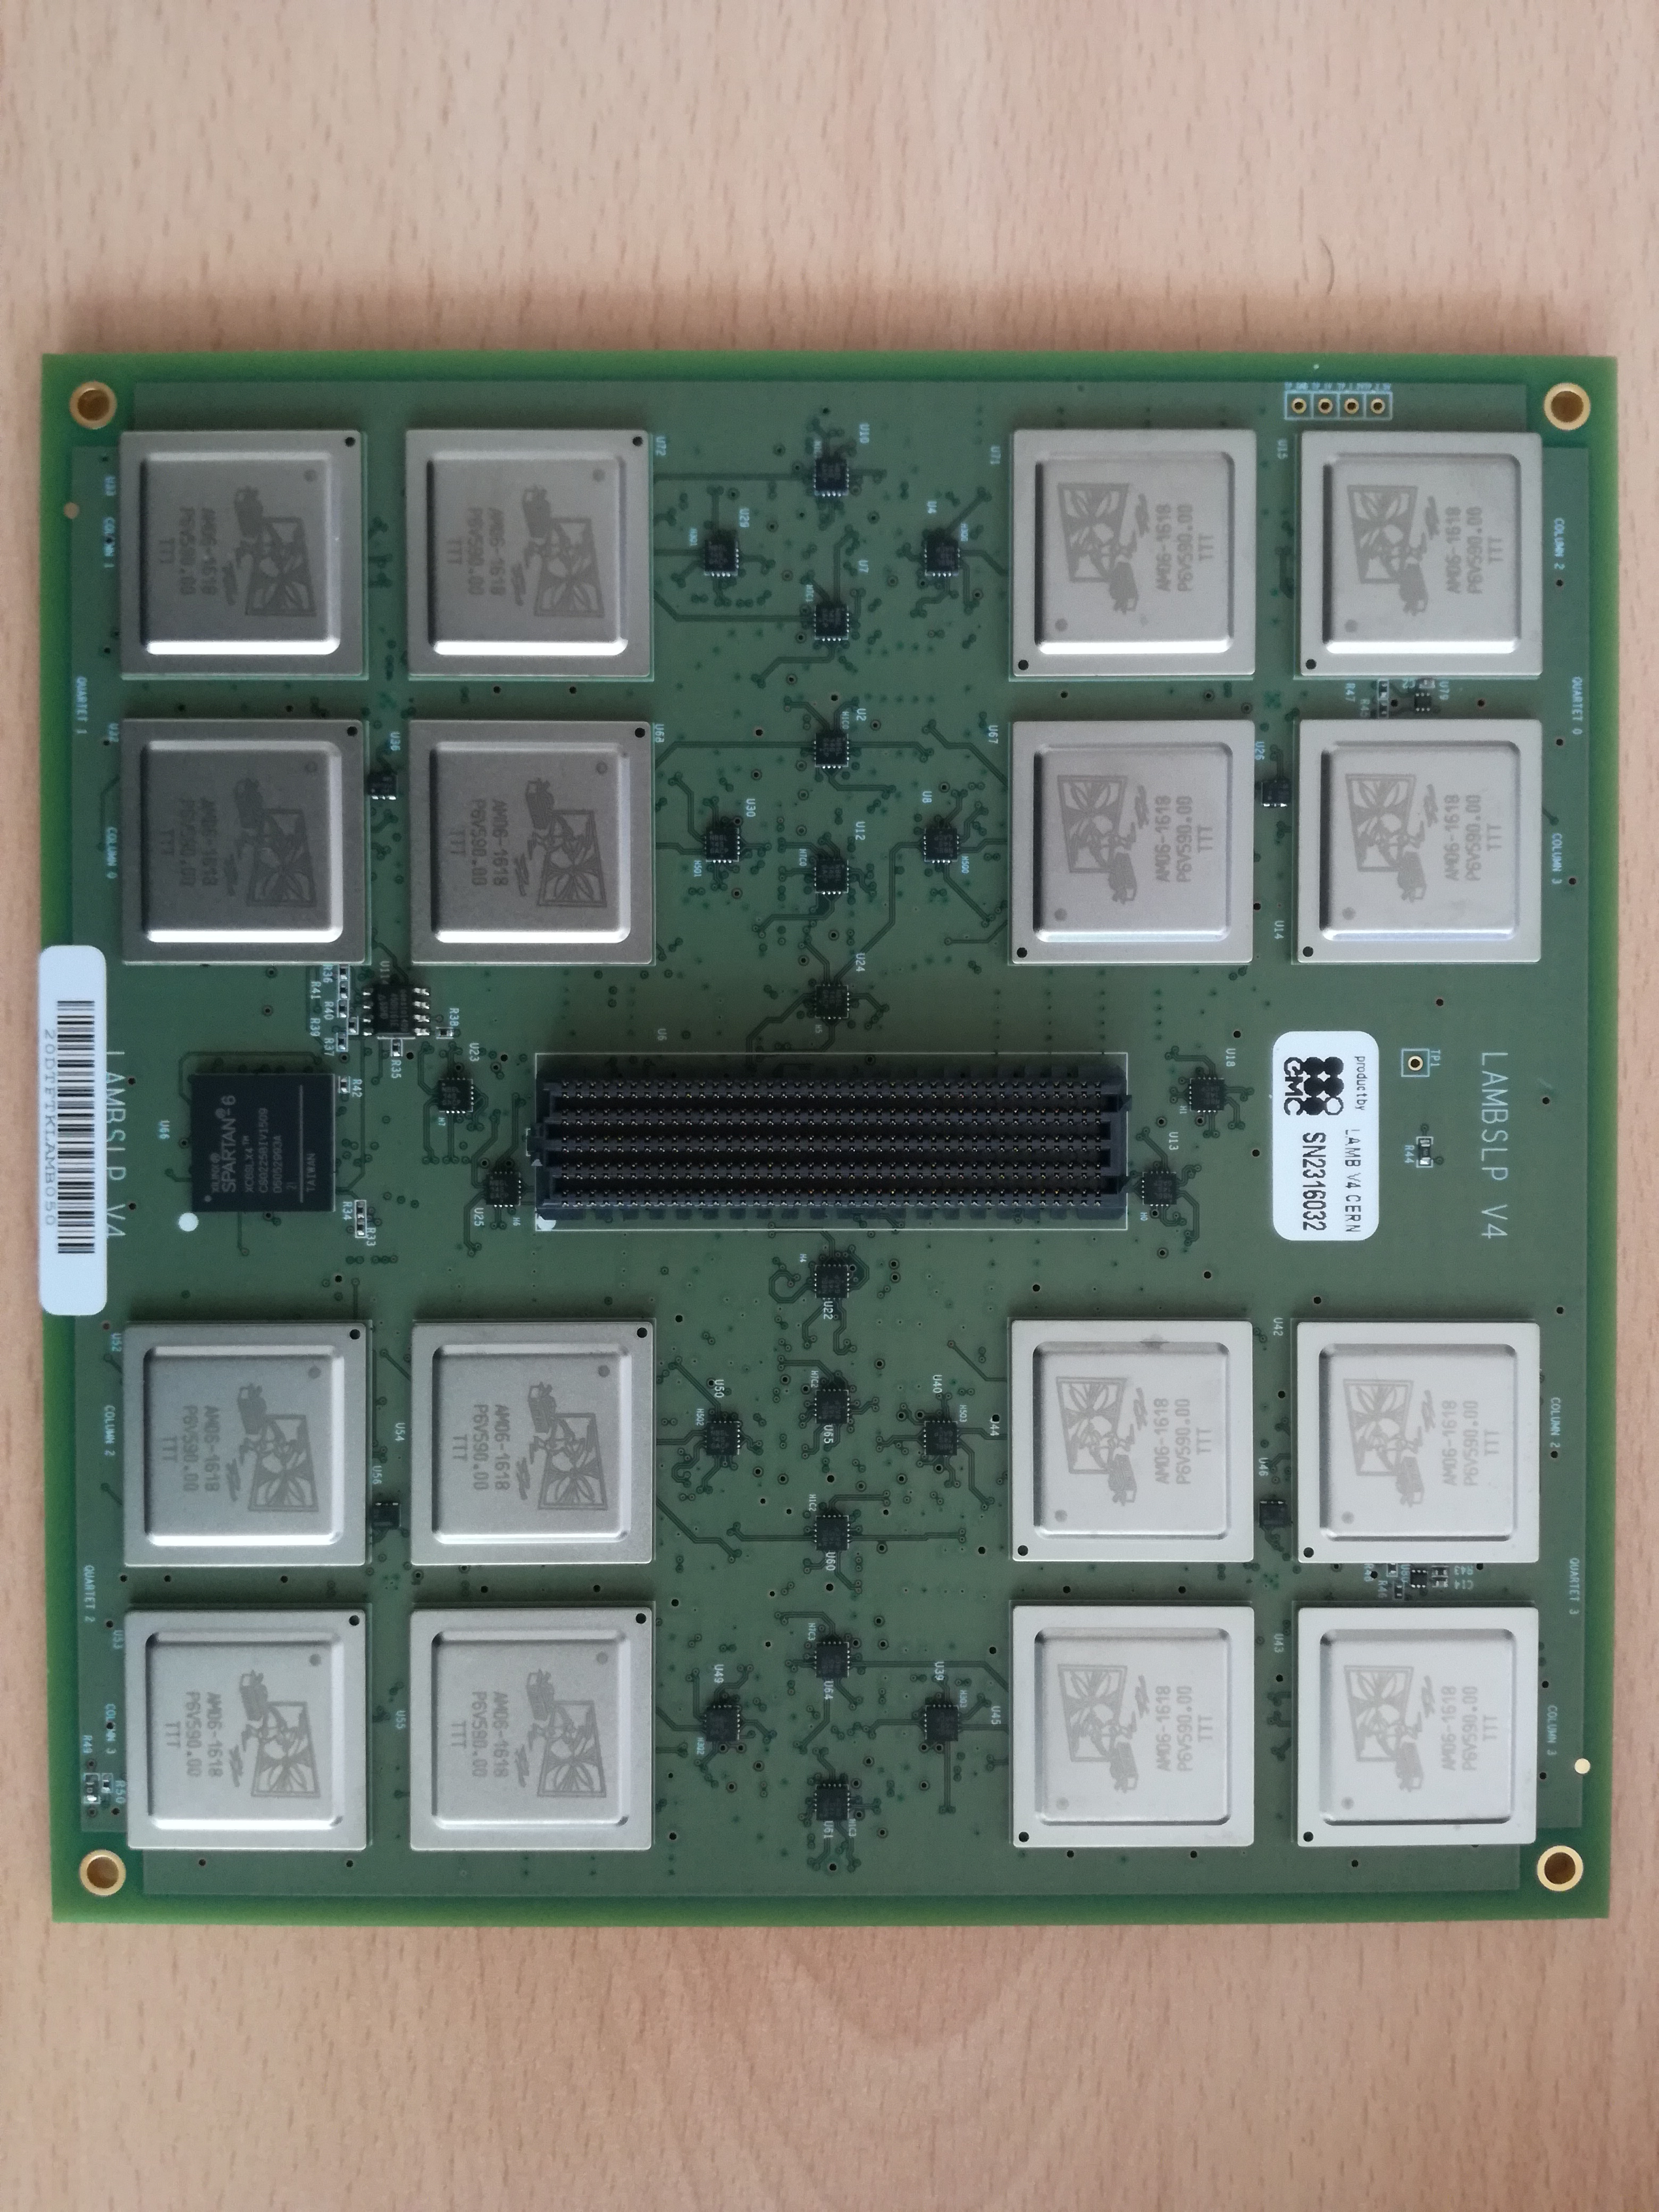
\includegraphics[width=.4\linewidth,angle=90]{Images/LAMB.jpg}

\caption{The figure shows a LAMB mezzanine, from the side that faces
the AMB and where the chips are installed. The organization of the chips
as quartets and the fan-out chips are clearly visible. The BUSCA
chip (Spartan VI FPGA) is installed below the FMC connector.}

\label{fig:lamb_bottom}
\end{figure}

The \AMBoard is a VME 9U board composed by 4 FPGAs and up to 4 extension cards,
the little associative memory boards (LAMB). The two cards are showed in 
Fig.~\ref{fig:amboard_top} and \ref{fig:lamb_bottom}.

The board loads a pattern
bank on the AM chips installed within the LAMBs, then receives input data
from the auxiliary (AUX) card installed on the back of the VME crate that are
distributed to the chips, performing a pattern recognition between the 
input data and loaded patterns. In this setup a pattern is an 8 16-bit array
of unsigned integer, each element is commonly referred as super-strip (SS)
or hit. 

\subsection{Board setup and control generalities}

\subsection{Input and output distribution and monitor}

The board receives input through the ERNI connector

\subsection{Chips configuration}
\label{sec:chipconfig}
 TODO
 
The AM06 chips show a configuration problem that causes loss of all matched
roads in an event, because of internal timing problem. To monitor this issue a
small test procedure: a special pattern is written in a known location, currently
position 0 within the chip, and has to fire at every event. A FW module counts in
how many events the test road was missing for each AM chip, indicating a problematic
configuration.
A loop of events can run for 1 second during the board 
bootstrap, all chips that show the incorrect behavior need to be reconfigured.
The procedure can be iterated fro a few times, until no faulty chips remain.
To cause the test pattern to fire this uses the WC value in all the layers,
because this SS value is sent at every event the road will be found with bitmask
$0xff$, if missing the chip had a failure.
 
\subsection{Power control and dummy hits}
\label{sec:powercontrol}

One of the most important characteristic of the board is the ability to distribute
the power to the AM chips. This is done by 4 DCDC converters, distributed on the
board near each LAMB, that are able to provide up to 80 A at $1\div1.2$ V. The
DCDC converters voltage and power can be monitored, and programmed, from the software
trough a set of VME commands.
To control the DCDC converters a PMBUS communication is used between the VME
FPGA and the DCDC converters. The PMBUS communication is implemented through the
VME interface using regular write and read requests, included in higher
level tools for convenience.

A second feature of the board related to the power need of the AM chips is
the so called \emph{dummy hit}. This is a special input word, created by the board
and sent to chip in place of normal idle words. This special input data cannot 
result in any match, or change the matching status of the patterns, however while
propagate through the chips it causes a controlled power consumption, function of
the number of bits swapping. Forcing the chips to have a not negligible power
consumption while not data are sent reduce the jump required by the DCDC convert
when real data arrive, improving the voltage stability and avoiding possible
issues due to voltage's ripples. The power consumption is a function of the 
bits changing between the first and last 16 bits, as example setting the dummy 
hit word as $0x0000ffff$, in the chip will be propagate 2 16-bit words: $0x0000$
and $0xffff$, 16 bits will swap from a word to the next. 
More bits are swapping larger will be the  power consumption induced during idle
periods. During the idle period the dummy hit is alternated with real idle words,
not causing bit swap in the chip, the ratio between the two type of data can also be
set.

\section{Configure and control the board standalone tools}

The status of the board is controlled by reading VME registers, associated
to the various.

\subsection{Control the board status}
To control the board status the main available command is
\textbf{\texttt{ambslp\_status\_main}}\index{ambslp\_status\_main}. 
This should be
launched from the VME SBC or in a node where the ATLAS Information
Service (IS) available.

The command line options are limited. The most important are the \textbf{slot} 
number, used to set the VME slot where the board in installed and
the partition name, used to eventually retrieve the board
information from IS.

In both cases the output is printed on the screen and can be quite 
verbose, for this reason an example will be presented here in
pieces.

\begin{itemize}
	\item The first part reports if the data are from IS or not and the
	firmware version uploaded into the FPGAs:
	\begin{verbatim}
	++++++++++++++++++++++++++
	ambslp_status(), read from IS:
	0Hit Firmware version:  0xd220a7df
	CONTROL Firmware version:  0x4
	VME Firmware version:  0x521
	ROAD Firmware version:  0x2a210413
	\end{verbatim}
	in case of problem  the firmware version  can be 0xffffffff or 0x0, 
	both values are commonly related to a configuration issue.
	
	\item The following part reports the temperature on the LAMBs:
\begin{verbatim}
++++++++++++++++++++++++++
Temperature measurements
VME slot front | LAMB2 | LAMB2 | LAMB0 | LAMB0 | VME back plane
VME slot front | LAMB3 | LAMB3 | LAMB1 | LAMB1 | VME back plane
|    0  |    0  |   34  |   32  |
|   28  |   29  |   29  |   28  |
\end{verbatim}		
	the reported values are organized in rows and columns, reporting
	the geographical organization of the LAMBs within the AMB. A $0$
	temperature usually means that no card is installed in a specific slot,
	$255$ means that the sensore is not instlled or not working,
	better information can be assessed checking for the board information
	into EDMS.

	\item The following bloc reports the status of the HIT FPGA. At the
	begin of this long output section the eventual test-mode (TMODE) and
	PLL locks are reported, the presence mask of the LAMBs, then hold and 
	empty status for the input FIFOs.
	for the links
\begin{verbatim}
++++++++++++++++++++++++++
HIT STATUS
TMODE:           1
PLL lock:        f
PLL REF LOCK:    0

LAMB mask:  f00

SCT hold status:  0
PIX hold status:  a6

SCT empty status:  6
PIX empty status:  0
\end{verbatim}
	The presence mask is a 4-digit number where \textbf{0} means the 
	\emph{card is present}, \textbf{f} the \emph{card is missing}, the
	example can be read as f00=0f00, that means LAMB 2 is missing.

	\item The next portion of the HIT report section represents the
	alignment of the serial links to the chips and the AUX.
\begin{verbatim}
GTP align QUAD216:  1 - 1 - 1
GTP align QUAD213:  1 - 1 - 1
GTP align QUAD116:  1 - 1 - 1
GTP align QUAD113:  1 - 1 - 1

GTP reset done QUAD 216 RX:  f - TX f
GTP reset done QUAD 213 RX:  f - TX f
GTP reset done QUAD 116 RX:  f - TX f
GTP reset done QUAD 113 RX:  f - TX f
\end{verbatim}

	\item The final part of the HIT summary shows the HIT FSM satus,
	useful in case of debugging of the board, the input rates and the number
	of errors in each link.
\begin{verbatim}
HIT SCT FSM status: 0x1121
HIT PIX FSM status: 0x1111

ch 0    ch 1    ch 2    ch 3    ch 4    ch 5    ch 6    ch 7   ch 8     ch 9    ch 10   ch 11
HOLD  1s        5e-08   4e-08   4e-08   4e-08   1.51812 0.00133648      1.5059 0.00656278       1.51965 0.00053916      1.50891 0.0108022
EMPTY 1s        1.51084 1.51084 1.51085 1.51086 2.38e-06        1.09e-06       2.49e-06 1.05e-06        2.25e-06        1.16e-06        2.31e-06        1.04e-06

Lost of Sync error counter. For each link count 0-255 and then wrap around.
SCT link 0:    00
SCT link 1:    00
SCT link 2:    00
SCT link 3:    00
PIX link 0_0:  00
PIX link 0_1:  00
PIX link 1_0:  00
PIX link 1_1:  00
PIX link 2_0:  00
PIX link 2_1:  00
PIX link 3_0:  00
PIX link 3_1:  00
\end{verbatim}

	\item The next part of the staus represents the CTRL FPGA, where
	the FSM state in controlling HIT and ROAD FPGAs are reported. The
	block is self-explanatory
\begin{verbatim}
++++++++++++++++++++++++++
CONTROL STATUS
Firmware:        15 v.4
FSM state Hit:   1
FSM state Road:  2

Control FSMs are documented in Figure 4, section 1.2.1 of the AM board documentation.
FSM state HIT:  0 = wait for initial global init
1 = send hits event N; wait for HIT end event on all channels and for DONE ROAD previous event
2 = wait X cycles
3 = DONE HIT event N, send INIT_EV
4 = wait a few cycles
FSM state ROAD: 0 = wait for initial global init
2 = DONE ROAD event N-1
1 = send ROAD to AUX event N-1
3 = wait a few cycles
\end{verbatim}

	\item The following block of messages refers to the ROAD FPGA. 
\begin{verbatim}
++++++++++++++++++++++++++
ROAD STATUS
Firmware:      14 v.1
TMODE:         0
PLL lock:      f
PLL REF LOCK:  0

Hold Aux status:  0

Empty Fifo Lamb_0 Status:      f
Empty Fifo Lamb_1 Status:      f
Empty Fifo Lamb_2 Status:      f
Empty Fifo Lamb_3 Status:      f

Prog Full Fifo Lamb_0 Status:  0
Prog Full Fifo Lamb_1 Status:  0
Prog Full Fifo Lamb_2 Status:  0
Prog Full Fifo Lamb_3 Status:  0

ROAD input link UP QUAD216:  c
ROAD input link UP QUAD213:  f
ROAD input link UP QUAD116:  c
ROAD input link UP QUAD113:  f

GTP reset done QUAD 216 RX:  f - TX f
GTP reset done QUAD 213 RX:  f - TX f
GTP reset done QUAD 116 RX:  f - TX f
GTP reset done QUAD 113 RX:  f - TX f
\end{verbatim}
	The first registers
	report on the test-mode flag and the PLL locks. The eventual hold signals from the 
	AUX are also reported. The are then the registers related to the empty or full 
	status for the FIFOs that collect the output from each LAMB, 
	
	\item 
\begin{verbatim}
LAMB = 0
Missing patternX link 0 = 0x0 0x0 0x0 0x0
Missing patternX link 1 = 0x0 0x0 0x0 0x0
Missing patternX link 2 = 0x0 0x0 0x0 0x0
Missing patternX link 3 = 0x0 0x0 0x0 0x0
LAMB = 1
Missing patternX link 4 = 0x0 0x0 0x0 0x0
Missing patternX link 5 = 0x0 0x0 0x0 0x0
Missing patternX link 6 = 0x0 0x0 0x0 0x0
Missing patternX link 7 = 0x0 0x0 0x0 0x0
LAMB = 2
Missing patternX link 8 = 0x0 0x0 0x0 0x0
Missing patternX link 9 = 0x0 0x0 0x0 0x0
Missing patternX link a = 0x0 0x0 0x0 0x0
Missing patternX link b = 0x0 0x0 0x0 0x0
LAMB = 3
Missing patternX link c = 0x0 0x0 0x0 0x0
Missing patternX link d = 0x0 0x0 0x0 0x0
Missing patternX link e = 0x0 0x0 0x0 0x0
Missing patternX link f = 0x0 0x0 0x0 0x0
\end{verbatim}

	\item the final part of the \texttt{ambslp\_status\_main} output
	reports the disparity error: from the link:
\begin{verbatim}
LAMB0 RX 8b/10b or disparity errors = 0x0
LAMB1 RX 8b/10b or disparity errors = 0x0
LAMB2 RX 8b/10b or disparity errors = 0xffffffff
LAMB3 RX 8b/10b or disparity errors = 0x0
\end{verbatim}
	there is a 32-bit register available for each LAMB, the number is at
	the begin of the line, and the bits in the word represents the serial
	lines at had at least one disparity error. This bit can only be reset
	with a reinitialization of the board of levels 0 and 2,
	 see \ref{sec:ambslpinit} for more information.
\end{itemize}

\subsection{Initialize the board}
\label{sec:ambslpinit}

The AMB initialization is performed sending a specific command
to the board through the VME bus, this can be done using the 
\textbf{\texttt{ambslp\_init\_main}} program. The program has two
main options: the board slot (\verb|--slot--|)and reset level (\verb|--amb_lamb| 
or positional argument).
Examples of the command line are:
\begin{verbatim}
$ ambslp_init_main --slot 2 --amb_lamb <N>
$ ambslp_init_main --slot 2 <N>
\end{verbatim}

At the moment there are 4 initialization levels available:
\begin{description}
	\item[0] this performs a basic reset of the FSMs, eventual loops
	are stopped, FIFO content and configuration registers are unchanged.
	
	\item[1] this performs a reset of LAMB's FIFOs.
	
	\item[2] performs a cleanup of the AMB's FIFOs.
	
	\item[3] perfoms a full reinitialization of the configuration registers
	in the board.
\end{description}


\subsection{Configure the AM chips}



\subsection{Pattern bank setup}
\label{sec:bankload}

A pattern bank can be loaded from \ldots

\section{High-level procedures}
\label{sec:highlevel}

The tools describes up to now usually provide a low-level
interaction with the AM board, controlling a single feature
or asserting a single command at the time. It is however 
possible to perform high level procedures, composed by a sequence
of commands.

To perform this kind of operation the command line tool
\textbf{\texttt{\index{ambslp\_procedure}}} commands can be used. The
command line to run this tool will be similar to the
following:
\begin{verbatim}
$ ambslp_procedure [options] transition1 [transition2 ...]
\end{verbatim}
where the options block can specify parameters used by one, or more,
of the following \emph{transitions}. The optiosn are often in common
with other tools, already described, clarifications already by the emended help.
The \emph{transitions} are commands related to common procedures
that the board needs, the name are often in common with the
run control module. The transitions will be executed
sequentially, following the order in the submission string, they can 
be also executed multiple times.

Available transitions are described in deatails within the following 
subsections. The name of the procedures are often related to the run
control transition, more details in \ref{sec:rcmodule}.

\subsection{Configure the boards}
\label{sec:procconfigure}

The procedure keywords are \textbf{\index{ambslp\_procedure!configure}} or \textbf{config}  this procedure provide some basic configuration of the boards, should done every time a test start. It
    also configure the AM chips output and the GTP link from and to the
    ROAD FPGA.

\subsection{Loading a pattern bank}
\label{sec:procloadbank}
The keywords are \textbf{loadbank} and \textbf{load}, 
this command performs the
	sequence of operations required to write a pattern bank within
	the AM chips in the board. The parameters for the pattern bank 
	that will be written are decided through command line options.
	Used options: \texttt{bankpath}, \texttt{type}, \texttt{N}.
    
    The \texttt{bankpath} option allows to set the pattern bank
    file to be loaded. The path can be a special keyword that
    allows automatic bank generation, two types of banks are
    currently supported: \texttt{random}, generating a random bank,
    \texttt{seq[N]}, generating bank where all super-strip of
    a given pattern are equal and function of the pattern position
    of the chip following this formula: $SS[i] = i\%N$, where \% is
    the integer rest operator, i the pattern position within the chip
    and N the optional parameter passed after the \texttt{seq}
    keyword, if not specified this is equal to the number of patterns
    per chip loaded. \texttt{N}, or \texttt{nPattsPerChip}, sets
    the number of patterns per chip that will be loaded.

\subsection{Connect the boards}
\label{sec:procconnect}

The keyword is	\textbf{connect}, this connects transition
	of the ATLAS run control software, more explanation later, and
	performs the link synchronization for the chips' input busses and
	with the HIT FPGAs, also ensure the input links from the AUX
	are properly set.


\section{Debugging the board}

\subsection{Retrieve information from the spy-buffers}
An important tool to debug an \AMBoard while is working is to check the
spy-buffers content. A spy-buffer is a buffer that stores the last data words
received, or sent, by the board. In total there are 12 input and 16 output
spy-buffers. Three different softwares are available to obtain the spy-buffers
content: \textbf{\texttt{\index{ambslp\_inp\_spy\_main}}} is used to retrieve
the input spy-buffers, \textbf{\texttt{\index{ambslp\_out\_spy\_main}}} 
collects the output spy-buffers content, 
the most recent one is 
\textbf{\texttt{\index{ambslp\_spybuffer\_dumper\_main}}}, able to read
both input and output buffers and it will only tool maintained in the future.
More details on each program will be given in the following subsections.

\subsubsection{Input spy-buffers dump}

The \textbf{\texttt{\index{ambslp\_inp\_spy\_main}}} command
allows to obtain the content of the 12 input spy-buffers. The program 
requires a limited amount of options:
\begin{description}
\item[--slot num:] the slot number where the board is installed.

\item[--method num:] this allows to change how the spy-buffers content is presented,
more details later. Default is 0.
\end{description}

When used, the default behavior is to write on the screen a big table with 8192 rows
and 24 columns. The columns are organized in pairs, in 
each pair of columns the first represents the address in the buffer while the second
its content. Each row represents...

\subsubsection{Output spy-buffers dump}

The \textbf{\texttt{\index{ambslp\_inp\_spy\_main}}} command

\subsubsection{Spy-buffers dumper}
The \textbf{\texttt{\index{ambslp\_spybuffer\_dumper\_main}}} command includes
the functionalities of the previous two commands, with the advantage of allowing to
read the them in a synchronized way. Additional features are also available, as
the ability to store the information directly in files that can be used as input
for the board simulation or as input for a standalone test of the board, see
\pageref{sec:boardsim}.

\subsection{Check board with bitlevel emulation}
\label{sec:boardsim}
A small program emulating the board is available within the software
package. The board simulation program is 
\textbf{\texttt{\index{ambslp\_boardsim}}}. The goal of the program 
is compare a given input with the content of a pattern bank, as if loaded
by the real board, and predict list of the output roads.

An minimal example of how to use the simulation program is:
\begin{verbatim}
$ ambslp_boardsim -T 0 -N 131072 patterns.pbank.root sshits__L{0..11}.ss
\end{verbatim}
the first options are used to set the pattern bank type and how many
patterns should be loaded per chip, in this case all patterns in an AM06 chip.
The following arguments are the pattern bank file, in the same format
used to populate the chips of a real board, while the following files are
the list of input super-strips, here 12 files, 1 for each input link.
The simulation will save the list of output roads in a file named, by default,
\texttt{outroads\_sim.out}, having the same format of the output 
spy-buffer dump using method 2.

\section{Run control module}


The ATLAS run control (RC) allows a coordinated control of hardware and software
resources. The RC performs \emph{transition}, to which the resource reacts
performing specific operations, depending on setup configurations that can be
specified in a centralized service, the object key service (OKS). The RC commands
are interpreted as transition in a final state machine, all components are
expect to move to the same state responding to a request. Each item controlled
by the RC performs the transition without possibility to interact with other components.
In practice, to control a resource, in this case the AMB, there is the need of a 
\textbf{RC module} and at least one \textbf{OKS schema} file. The RC module describes
an objects that reacts to the specific transition of the RC FSM, while the OKS
schema represents the parameters that describe the RC module at runtime. Each 
AMB RC module has a related schema.

\subsection{Run control module implementation}
\label{sec:rcmodule}

The AMB RC module class is the \textbf{\RCModule}, inheriting
form the \texttt{ROS::ReadoutModule}. It reimplements the following
public methods: setup, configure, ... more details on the operations
performed in each commands are given in the following sub-sections.

\subsubsection{Setup}

This method reads the OKS configuration for the given \AMBoard, 
retrieving all the required keys. 

\subsubsection{Configure} 

The configure methods reacts to the \textbf{configure} transition of the RC,
and its performed as soon after the transition starts. The internal
operations are controlled by the RC\_configure high level procedure and
loads a pattern bank,
see page \pageref{sec:procconfigure} in \ref{sec:procconfigure}.

\subsection{The AMB schema files}

To describe an \AMBoard there are a few schema files that are available, 
it follow the documentation of all the attributes.

\subsubsection{ReadoutModule\_Ambslp schema file}

This file describes the parameters of \RCModule. It inherits from 
\texttt{ReadoutModule} and \texttt{ResourceSetAND}. It declares the following
attributes:
\begin{description}
\item[Name:] sets the module name, e.g. ``AMB-2-15''. No default value is provided.

\item[Crate:] a numeric identifier for the crate. Type u32, default: 0.

\item[Slot:] the slot number where the board is plugged. Type u32, default: 0.

\item[HITFWVersion:] firmware version expected for the HIT FPGA. If the
FW version doesn't match the configuration procedure fails. 
If the value is $0x0$ the check is not performed. Type u32, hexadecimal, 
default: 0

\item[ROADFWVersion:] firmware version expected for the ROAD FPGA. 
Type u32, hexadecimal, default: 0

\item[VMEFWVersion:] firmware version expected for the ROAD FPGA. 
Type u32, hexadecimal, default: 0

\item[CTRLFWVersion:] firmware version expected for the CTRL FPGA. 
Type u32, hexadecimal, default: 0


\item[LAMBFWVersion:] firmware version expected for the BUSCA FPGA each LAMB;
all installed LAMBs are expected to have the FW version. 
Type u8, hexadecimal,  default: 0.

\item[DryRun:] boolean flag, when true the RC module avoids to perform VME calls,
allowing the RC infrastructure to be tested even without boards. Type bool,
default: 0.

\item[ForceWrite:] boolean flag used to force the write of a pattern bank; when
false the bank checksum register is matched with the one of the bank in memory, then
patterns are then loaded only if the two don't match; when true the bank is realoded,
skipping the check. Type bool, default: 0.

\item[DummyHit:] this represents the value of the \emph{dummy hit} word registers,
if the value is $0x0000000$ the feature is disabled, if not a dummy hit loop is
started during IDLE periods, as explained in \ref{sec:powercontrol}. Type u32,
default: 0.

\item[DCDCSetVolt:] this value is used to set the DCDC voltage output to the
desired value, as some relation with the resistors mounted on the DCDC. Type u32,
hexadecimal, default $0x02e3$ (1.15 V output on AMBv5).

\item[DCDCScale:] value used to convert the voltages obtained from the DCDC
check in volts. Type float, default $1.6666666666666667$.

\item[AddTestPattern:] boolean flag that controls the writing of the test pattern,
assumed to exist in every chip (see Sec.~\ref{sec:chipconfig}). If true a test
pattern is forced in the chip's position 0, patterns loaded by the user will start from
position 1 in the chip. If true the available space for patterns will be
reduced of 64, because 1 special pattern per chip will added by the procedure.
If false the pattern bank from the user will be loaded as it is.

\item[OverrideSpecialPattern:] boolean flag that control the special pattern
SS values overwriting the SSs of the original bank, this implicitly assumes 
that the pattern bank has been prepared respecting this board constraint.
Type bool, default 1`.'

\item[DumpFolder:] path where dump files are saved. Currently unused.

\item[LAMBMask:] 32-bit hexadecimal mask that stores where which LAMBs are expected
to be present in the board, this is used to eventually stop the configuration
if the expected boards are not installed.

\item[InitialThreshold:] threshold used during the pattern bank loading. Type u32,
decimal, default 15.

\item[Threshold:] pattern matching threshold. Type u32, decimal, default 7.

\item[CheckBank:] flag that enables the possibility to check the bank content
through JTAG. The procedure is extremely slow and not performed by default.
Type bool, default 0.

\item[BypassBus:] unused. Type u32, hexadecimal, default 0x24.

\item[PCBVersion:] unused. Type u32, decimal, default 0.

\item[DVmajority:] unused. Type boolean, default 0.

\item[Extras:] array of strings, with dynamic size, that can be freely used by the code.
The key is provided to allow to have unexpected parameter in the code in all cases
where a new schema cannot be deployed, e.g. quick code patches. The parsing of the
field is expected to be strongly dependent from the code tag.

\item[PatternBankConf:] link to an OKS object of the \textbf{PatternBankConf} type,
see Sec.~\ref{sec:pattbankschema}. This objects describe the location of the pattern
bank to be loaded in this bank, if no object is provided the configuration stage
of the \RCModule will fail.

\item[AMBStandaloneTest:] standalone test object, defined in Sec.~\ref{sec:ambtestschema}.
When an object on this type is set the \AMBoard is expected to load test-vector
data from the HIT input FIFOs instead of expecting data from the AUX. If no
object is provided the test is not performed.
\end{description}


\subsubsection{PatternBankConf schema}
\label{sec:pattbankschema}

\subsubsection{AMBStandaloneTest schema}
\label{sec:ambtestschema}

This schema represents the input parameters for an \AMBoard standalone test.
This kind of tests reads data from the HIT FPGA input FIFOs instead of waiting
them from the AUX. During this tests, AUX data will be rejected, while the
output can reach the AUX.

\begin{description}
	\item[TestFilePath:] this is the path of the file containing the data to
	be loaded into the board. The path has to be accessible from the RCD application,
 indeed	from a path available in SBC computers of the crate, where the board is used,
 or a network path, eventually public. Type string.
 
 \item[Loop:] boolean flag that controls if the data are sent only once or
 in a continuous loop. The loop has to stopped through RC or generally sending
 an init to the board. Type bool, default 0.
\end{description}

\section{AMBoard class and library structure}
\label{sec:library}

The \texttt{ambslp} package is mostly written in C++, requiring C++11 
compatible compilers. It defines the \textbf{\AMBoard} \index{AMBoard!class} and other low
level function able to communicate, to spy or change the state of the board.
Most of the 

\section{Extra tools}

\subsection{Upload firmware on the board}

It is possible to upload firmware on the board using SVF files,
produced using Xilinx Impact or other software, in the board
using the VME interface. An intrinsic limitation of this procedure is
that the firmware of VME FPGA cannot be changed.

The procedure is based on the creation an SVF file, the SVF file can then
be used by a specific program that send uses those information to reprogram
the FPGAs: \texttt{\index{ambslp\_svfplayer}}. The SVF file an contain information
to reconfigure the FPGA, reprogramming the flash memories or other
common operations, as reading the ID codes.

\subsubsection{Create the SVF file using Xilinx Impact}
To create the SVF it is necessary to open the Xilin Impact software. In case
the computer is connected to an \AMBoard scan the cable and remove the 
first FPGA in the JTAG chain, this is the VME FPGA and is not available
within the JTAG chain seen during the remote programming procedure.

An Impact project with the right JTAG chain is available in the firmware
repository \href{https://svnweb.cern.ch/trac/atlasftkfw/browser/AMboard/trunk/AMBSLP/AMBv4_vmechain.ipf}{\texttt{\textbf{AMBv4\_vmechain.ipf}}} and can be opened in impact to generate the SVF
files.

After the chain is modified, and reflects the needs for remote programming,
the proper bitstream and flash files can be assigned to the components in the
chain. It is not necessary to edit all elements, the general rule is in fact to
provide a specific SVF file for any major FPGA configuration.

To create then an SVF file go to the menu 
``Output>SVF File'', then click on ``Create SVF File''. Choose a position and
a name for the output file, a dialog box with an information message will appear,
as well as a blue text on the top right corner of the impact. More messages on the bottom
status bar will repeat that Impact is in SVF mode. Perform then all the operations
you would do as if a regular cable is plugged. All output will be sent to the file,
instead to the actual devices. Multiple operations can be done in the same sessions.
When the all commands are sent go in the SVF file menu item and close the file.
window will appear confirming that the 
While the SVF file receives the commands multiple operations can be performed,
it is common to perform only a major operation per session, e.g. program a single
FPGA or a single SPI FLASH memory, read the ID codes\ldots.


\subsubsection{Remote programming \AMBoard and LAMBs}

The program to be used to perform the remote programming, or other operations
on the FPGA chain, for either the mainboard
or the LAMBs is \textbf{\texttt{\index{ambslp\_svfplayer}}}. The program has to
be executed in the SBC where the board to be programmed is installed and has
a very simple command line. Available options are:
\begin{description}
\item[--slot num:] set the slot number where the board to be configured is
plugged, default 15.

\item[--svffile, -S file:] this option sets the SVF file(s) to be executed to
configure the FPGAs. The option can be used multiple times, all files will be
executed, in the order they appear in the command.

\item[--lamb, -l:] if present the operations in the SVF file(s) will be sent
to the LAMBs.

\item[--bt, -B:] if present the communication with the board will use the 
VME block-transfer mechanism.

\item[--nocomment, -N:] if present the comments in the SVF file are not
showed in the output.

\item[--verbose, -v num:] set the default level, increasing or decreasing
the amount of output information, default 1.
\end{description}

An example of the use for the program is the following:
\begin{verbatim}
$ ambslp_svfplayer -S test_idcode_amb.svf
Begin of programming sequence for AMB
Comment:  Created using Xilinx Cse Software [ISE - 14.7]
Advance 1% read 50 of 2902
Total number of bits: 0
Total number of TDO errors: 0 (Tot checks 0)
Total RUNTEST IDLE time 0 secs, Tcks 0
Comment:  Date: Wed Oct 19 16:14:49 2016
...
Advance 99% read 2873 of 2902
Total number of bits: 661
Total number of TDO errors: 0 (Tot checks 9)
Total RUNTEST IDLE time 0 secs, Tcks 0
ALL GOOD
Switching off programming for AMB

Elapsed time: 0 seconds
\end{verbatim}
in this case the default slot is implied for the board and a simple
SVF file that reads, and verifies, the ID code of the installed FPGAs is used.
This operation is used during the board testing to verify a good 
communication between the VME FPGAs and the JTAG chain. 

The software performs a check of the TDO signals, allowing to verify
that the output messages from the JTAG commands in the SVF file are as
expected. An ALL GOOD message is visible in the final part of the program.
In case of mismatches in the TDOs are met, their number is reported, the
exit status of the program is 0 if all TDOs match the expectation, -1
otherwise.

SVF files generated by Impact usually contain comments, used to 
described specific steps of complex operations, i.e. during flash programming.
The player prints out those messages as they appear, allowing to monitor
how the advancement of the whole operation. Other messages that show
which fractions of the SVF file has been parsed are also shown, in this
case also the total number of bits sent to the JTAG chain is also 
printed, as well as a summary of the total TDO messages checked, and
eventual errors, until now.
this point 

\appendix
\section{Common example}
\subsection{Configure the board with a random bank}

\begin{verbatim}
$ ambslp_procedure --slot 15 --bankpath random configure load connect
\end{verbatim}

\printindex
\end{document}